\section{Body} \label{sec:body}


The body of your thesis usually consists of a sequence of sections and sunsections that tell the story of your problem, approach and results. 

We're using this section to exemplify some of the conventions you should follow for integrating figures, references etc.

\subsection{Motivation} \label{sec:body_motivation}

The world record in recalling historic dates is roughly equal to all the dates children have to learn during their entire time in school. The world record holder did it in five minutes while the average high-school student, looking back on their 12 years of education, is likely to remember no more than a handful of them \cite{how_to_become_a_memory_master}. It took Zou Lujian 13.96 seconds to remember the order of a shuffled deck of 52 playing cards \cite{record_recall_playing_cards}. When people are presented with these achievements they often assume only extremely rare geniuses could accomplish such tasks or perhaps think that aliens really are among us. To me that highlights a lack of awareness of the surprisingly simple techniques that are being used by all of these aliens. It also emphasizes how little we trust our ability to remember. "If you don't know the information is there, you don't trust your brain. If you don't trust your brain you study all the time."\cite{how_to_become_a_memory_master}. This quote reminds me of the distress I've felt before taking exams that involved a lot of memorization during my time in school. I've heard of people puking before medical exams and it is not surprising to me when I think of my sister's condition before she had her preliminary medical exam. I'm sure people can relate to this. Following what techniques enable the average person to trust their brain and if they are so simple and effective why are they not ubiquitous? We call those techniques \emph{mnemonics} and their usage dates back far beyond the Ancient Greeks \cite{white_2014}. Simonides allegedly helped to identify bodies of a collapsed building as he had remembered every person in a large banquet hall of the building by using a mnemonic device that we call today \emph{loci}. As the word loci suggests, it works by imagining a familiar place in one's mind and associating parts of that place with words from e.g. a shopping list or in the rather peculiar example of Simonides, a group of people. If your're list requires ordering you can use the \emph{peg system} where you first must memorize a list of distinct objects after which you could associate each item on the list with e.g. the first 10 presidents of the US. If there is a mnemonic device that is known to almost everyone, it is probably \emph{acronyms}. You may use or have used \emph{soh cah toa} to remember ratio formulas of triangles. Although these methods may already inspire curiosity in the field, it's quite a leap to think that people can remember up to 70000 decimal places of \emph{pi} by using them \cite{record_decimal_pi}. Alongside an insatiable desire to learn things that are arguably useless, except for impressing the public, there must be another layer that closes the gap between techniques described so far and remembering inherently abstract things like numbers. This can be achieved by using \emph{phonetic systems}. The method utilizes a table that maps numbers to consonants that can then be employed to form words. The word \emph{cup} for instance translates to the number \emph{79} with the so called \emph{major system} \cite{major_system}. Subsequently you turn numbers into words and words into stories to remember the entire sequence. While this may be used to recall the number of your close ones the next you are lost in the wild without a phone, with enough practice, you may start aspirations to break the record in recalling decimal places of pi. Another common technique is the \emph{keyword mnemonic} that steps out of the memory athlete realm and shines with more practical applications most commonly found in second language learning. The process involves finding a keyword that is phonetically similar to the one the student wants or perhaps more accurately is obliged to learn and then form a sentence or phrase that connects the two words in a meaningful manner. E.g. the Japanese word 食べる (taberu) meaning \emph{to eat} sounds like the word \emph{table}. Following one could come up with a phrase like so: "Imagine you eat your lunch on the table. You wouldn't eat on the floor. That's inappropriate!". It seems only natural to assume that given their incredible success among memory athletes mnemonic devices should be everywhere in education. Evidently they are almost nowhere in traditional education except for a few acronyms here and there. To unwrap that conundrum it is worth looking into existing research on the topic. Most of the research I have come across tests the effectiveness of mnemonics in education by comparing groups that use mnemonics with groups that do "nothing", or at least do nothing special to recall the given material. Because of it's application in second language learning keyword mnemonics are a common choice for these comparisons. Ample such studies suggest that the use of mnemonics in education significantly improves academic performance while others do not \cite{putnam_2015}. This may be due to the simplistic nature of conducted studies as they often neglect the fact that the control group is already using mnemonic devices, whether participants are aware of it or not, as has been shown by \cite{the_do_nothing_group} explaining \emph{what the "do-nothing" group does}. Additionally mnemonic devices have been criticized to be no better than more straightforward methods like repetition and taking notes when it comes to long-term learning \cite{putnam_2015}. To assume that there exists a learning method that lets individuals engrave information into their brain like a read/write head does on a hard disk is preposterous. It is important to note that mnemonics can enhance learning but still require repetition. Furthermore I argue that mnemonics are a much more engaging and fun way of learning and given that groups utilizing mnemonics almost always outperform the control groups in immediate retrieval \cite{putnam_2015} of the learned material, I find it reasonable to suggest that learning with mnemonics also saves time. Most importantly mnemonics can help individuals to regain trust in their brain's ability to recall information which also reduces anxiety in students as they have a sort of legal "cheat sheet" during exams \cite{putnam_2015}. Despite my appraisal of mnemonic devices they are still not found very often in the classroom or the everyday life. It's not very difficult to see the reason for the latter as we no longer have to rely on our brains to remember as much. White has pointed out that with Gutenberg's invention of the printing press mnemonic devices were swept off the table as information was now much more accessible. \cite{white_2014} The revolution that came with digital information and the internet of course only accelerated this development. And while using mnemonics to remember phone numbers of your close ones seemed very useful 20 years ago, the need for this has been virtually eradicated with modern smartphones.
I believe the lack of mnemonics in the classroom is due to the fact that using them seems to involve extra work or initial efforts like memorizing a peg list or finding an appropriate keyword. This in turn makes them rather unattractive for already unmotivated students.
I believe the latest developments in Artificial Intelligence can bring mnemonics back into the classroom. \emph{ChatGPT} has made the recent progress of large language models like \emph{GPT-3} accessible to the average person and it's potential to use mnemonics more effectively is inexhaustible. However I focus my work on the specific use case of learning Japanese \emph{Kanji}. Websites like \emph{Wanikani} \cite{wanikani} have been successful in teaching students Kanji with mnemonics. \emph{Radicals} are components that make up Kanjis and when you combine their meanings with the meaning of the Kanji at hand you can create a mnemonic story or expression that combines the meanings from the Kanji and its Radicals. I suspect that thanks to the provided handcrafted mnemonics from Wanikani the site has been a success and is backed by a strong community. 
\begin{figure}
    \centering
    \includegraphics[width=300pt]{example-image-a}
    \caption{Some big figure example with a very long text, to test the spacing in multi-line captions.}
    \label{figure:example_figure}
\end{figure}



\subsection{State of the art} \label{sec:body_state_of_the_art}

Here I will describe mnemonics and their usefulness as well as methods of evaluating generated text by language models but ultimately I will conclude that most of these methods are useless for my use case as they either have a reference text or they make use of human annotated data which I don't have the resources for.
\subsection{Relevant Features} \label{sec:body_relevant_features}
\subsection{Evaluation Data} \label{sec:body_evaluation_data}

As I will not conduct a user study my approach of for evaluating the metric will be to analyze the difference of the metric scores between distinct groups of mnemonics. I have in total gathered data from 4 groups. Good examples of mnemonics have been randomly sampled from 
\emph{wanikani.com} because their popularity should be evidence enough to indicate decent effectiveness. As I was not able to find examples for the low end, I instead opted to generated them with the only requirement that the input words are found in the output. I chose a GPT-2 model for this task.  Additionally, two more example groups have been generated using GPT-3 with different prompts, one asking the model to come up with a paragraph that must include input words and another that prompted it to output a mnemonic story based on the input words. A total of 760 mnemonics have been collected for evaluation. Following an example of each group is shown given the input words \emph{plow, drunkard and planting}. They are derived from the Kanji 栽 which means \emph{planting}.
\begin{description}
    \item[WaniKani] A \emph{drunkard} gets his hands on a \emph{plow} and starts \emph{planting} right away. Drunk people are surprisingly good at \emph{planting}, especially when they have machines to help them do it. Picture a drunk guy laughing and plowing a field and \emph{planting} seeds. He wouldn't do this if he was sober, but drunk people can't help themselves.
    \item[GPT-2]  This is a \emph{plow} \emph{drunkard}'s guide to \emph{planting} trees in your yard. If you don't know what I'm talking about, check out my previous post on the subject: How To Plant A Tree In Your Backyard (And Why You Should Do It). This time we'll be looking at different types of tree species and how they can
    \item[GPT-3 paragraph] The \emph{drunkard} stumbled out of the bar and made his way to the nearby farm, where he began to \emph{plow} the fields for the upcoming planting season. He worked tirelessly for hours, his mind foggy with alcohol, until the fields were ready for the \emph{planting}.
    \item[GPT-3 mnemonic] Once upon a time, there was a \emph{drunkard} who stumbled into a field with a \emph{plow} in hand. He decided to \emph{plant} some seeds he had found in his pocket, and with a few clumsy swipes of the plow, he was able to make some furrows in the field. With a satisfied smile, he watched as the seeds he \emph{planted} took root. 
\end{description}
For the GPT-3 prompts I used the \texttt{text-davinci-003} GPT-3 model which is the most powerful of its evolution at the time of this writing. The used prompts are listed below.
\begin{description}
    \item[Paragraph] Write a short paragraph that includes the following words: drunkard, plow, planting
    \item[Mnemonic] Write a short paragraph long mnemonic story that is based on and must include the words: drunkard, plow, planting
\end{description}
For the low end examples I used a 1.5B parameter version of GPT-2 \cite{radford2019language}. Since a non fine-tuned GPT-2 model is not very good in providing sensible output given similar prompts to the ones above, I had to use \emph{constrained beam search} in order to ensure the requirement of including all input words. Instead of just using the most likely token at each generation step given the previous tokens, commonly referred to as \emph{greedy search}, beam search keeps track of the $n$ most probable candidates at every time step and uses them as context for the next iteration \cite{kim2022guiding}. The constrained version of the method forces the tokens that must be included in the output as possible extensions of the previous tokens and divides candidates into so-called \emph{banks}. Each bank is defined by how many of the constrained tokens are included in the candidate. Following, the $n$ candidates for the next iteration are selected by round-robin, taking the most likely candidate from each bank until $n$ is reached. The banks are also sorted by how many of the constraint tokens they include in their candidates. The process is visualized in Figure \ref{figure:constrained_beam_search_example}.  
\begin{figure}
    \centering
    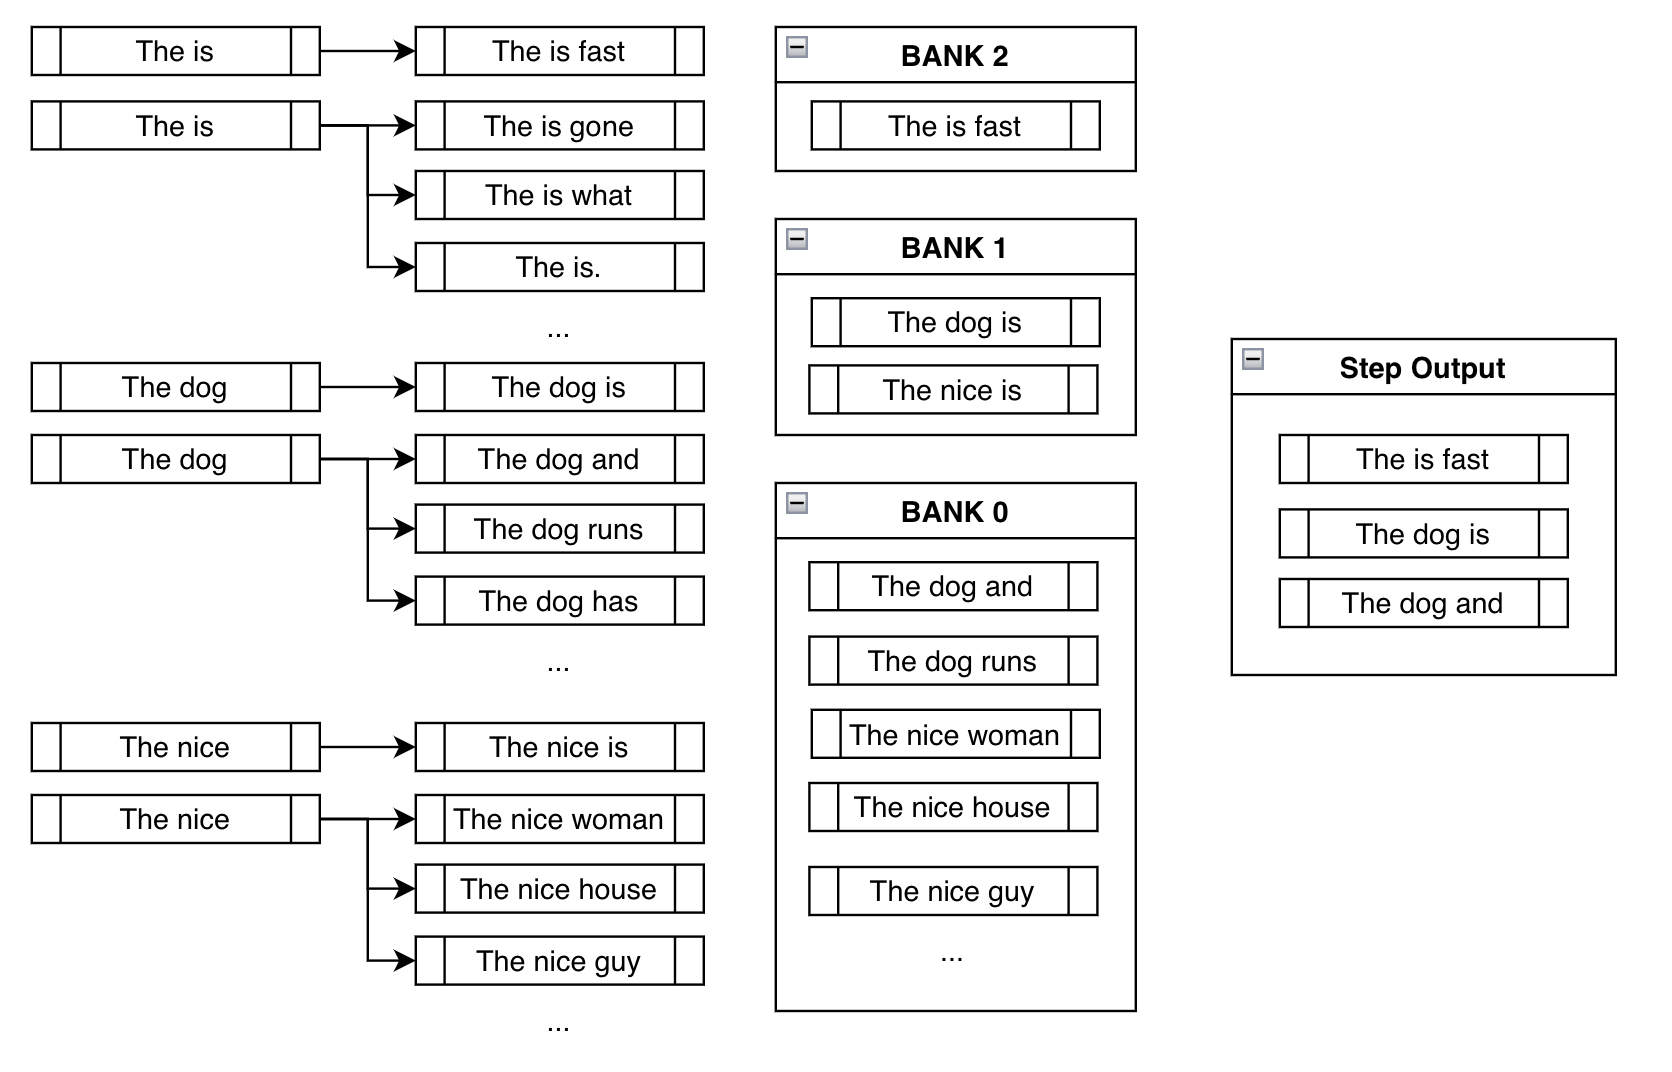
\includegraphics[width=400pt]{resources/cbeam_2.jpg}
    \caption{Constrained beam search example with forcing the phrase "is fast" \cite{kim2022guiding}}
    \label{figure:constrained_beam_search_example}
\end{figure}
\subsection{Feature evaluation} \label{sec:body_feature_evaluation}

Concluding chapter \ref{sec:body_relevant_features} I have identified the following features that describe effective mnemonics. 
\begin{enumerate}
    \item word vividness (imageability, concreteness)
    \item bizarreness of mental imagery
    \item centrality of input words with strong connections in the output
\end{enumerate}

Given the existing research it is plausible to start with quantifying the vividness of the mnemonics. It would be perhaps most plausible to train a model that outputs a score that captures the vividness of the input text. Unfortunately I was unable to find such data. In the field of psycho-linguistics however norms of words exist. Several datasets are available that incorporate human word scores for different norms. Norms relevant to my research are: imageability, concreteness and sensory modality. The latter seems useful as words that are strongly identified with different senses are likely to be very concrete and contribute to vivid imagery. One limitation that quickly emerges is that these datasets tend to be rather small and using them on their own won't cover enough words to be used effectively. Several successful attempts have been made to extend these norm datasets by training models that identify features from word embeddings \cite{concr_embed_bert, img_concr_svm, fusing_ctx_embed_concr}. \cite{concr_embed_bert} referred to research showing that concrete word embeddings tend to cluster with other concrete ones while abstract ones show the same general behavior. This is not surprising as embeddings from increasingly sophisticated models encode features of text extracted from enormous corpora. I mostly copied the architecture described in their paper to fine-tune DistilBERT for the regression task of predicting a concreteness scalar $c \in [0,1]$. In addition to the generous dataset of 40000 human concreteness ratings \cite{40000_concr} I trained the model with another 60000 multi word expressions from \cite{60000_concr}. This allows me to evaluate phrases rather than just words of the mnemonics in terms of concreteness. The fine-tuned model achieved a Pearson correlation of $0.88$ with the test data. Ten percent of the dataset had been used for testing. While this result is good the models of the paper performed up to $0.92$ in correlation. This gap in performance could be explained by the additional dataset used on my part. I suspect that it becomes less trivial to assess concreteness adding multi-word expressions to the training data. To support that point I have fine-tuned BERT as described in the paper with just using the 40000 word ratings. This model achieved a Pearson correlation of $0.918$ which is close enough. On a side note I hypothesized that more recent models like CLIP are perhaps better suited for the task of predicting concreteness as they form embeddings from text combined with images. My idea is that more abstract terms are in a different embedding space than concrete ones because they tend to have less distinct images associated with them. The set of possible images for the word \emph{cow} is probably a lot smaller than for the word \emph{female}. To investigate this I've compared CLIP with BERT on predicting word concreteness. Two models for each architecture had been trained. One that fine-tuned all weights while the other one froze all weights except for the regression head. This gives us an idea of how well the raw embeddings are at predicting concreteness. It may have been more appropriate to use imageability ratings for this comparison but since imageability and concreteness are related and the existing data for the latter is far more abundant, I chose to use concreteness ratings for this task. 
\begin{table}[ht]
\centering
\begin{tabular}{@{}lcc@{}}
\toprule
Model & Unfrozen Weights & Frozen Weights \\ \midrule
BERT           & 0.918                     & 0.752                   \\
CLIP           & 0.905                     & 0.800                   \\ \bottomrule
\end{tabular}
\caption{Pearson correlations for BERT and CLIP with unfrozen and frozen weights.}
\label{tab:clip_bert_comparison}
\end{table}
As expected (see Table \ref{tab:clip_bert_comparison}) the CLIP model with frozen weights outperformed the BERT version, however it strikes me as surprising that the opposite effect was observed in the case of fine-tuning all weights. This may be explained due to architecture differences and would require further research.

Two more DistilBERT models have been fine-tuned to predict imageability and sensory modality scores. The latter was trained with 1792 examples \cite{Juhasz2013} gathered from participants that where asked to rate the degree to which each word evoked a sensory experience. The MRC psycholinguistic database \cite{mrc} contains 4828 imageability ratings which I used to train the first model. The models used for evaluating mnemonics and their test results are displayed in Table \ref{tab:linguistic_features_pearsonr}.


\begin{table}[ht]
\centering
\begin{tabular}{@{}lc@{}}
\toprule
Models          & Pearson Correlation \\ \midrule
Concreteness             & 0.880                        \\
Sensory Modality         & 0.706                        \\
Imageability             & 0.875                        \\ \bottomrule
\end{tabular}
\caption{Pearson correlation coefficients for the fine-tuned DistilBERT models}
\label{tab:linguistic_features_pearsonr}
\end{table}
Perhaps the most straightforward way to evaluate the mnemonics is to take the mean (Equation \ref{eq:token_mean}) of the word scores from the individual models.
\begin{equation} \label{eq:token_mean}
    s_{\text{mnemonic}} = \frac{1}{N}\sum_{w=1}^{N}\text{model}(w)
\end{equation}
I consider only words that are not labeled as stopwords. The results for sensory modality, imageability and concreteness are shown in Tables \ref{tab:mean_std_ser}, \ref{tab:mean_std_img}, \ref{tab:mean_std_concr} and Figures \ref{figure:ser_mean_box_plot}, \ref{figure:img_mean_box_plot}, \ref{figure:concr_mean_box_plot} respectively.
\begin{table}[ht] 
\centering
\caption{Means and Standard Deviations for Sensory Modality}
\label{table:group_stats}
\begin{tabular}{lcc}
\toprule
Group & Mean & Standard Deviation \\
\midrule
GPT-2& $0.337$ & $0.043$ \\
GPT-3 (mnemonic) & $0.320$ & $0.055$ \\
GPT-3 (paragraph)& $0.351$ & $0.065$ \\
WaniKani & $0.347$ & $0.063$ \\
\bottomrule
\end{tabular}
\label{tab:mean_std_ser}
\end{table}

\begin{table}[ht] 
\centering
\caption{Means and Standard Deviations for Imageability}
\label{table:group_stats}
\begin{tabular}{lcc}
\toprule
Group & Mean & Standard Deviation \\
\midrule
GPT-2& $0.558$ & $0.043$ \\
GPT-3 (mnemonic) & $0.569$ & $0.054$ \\
GPT-3 (paragraph)& $0.583$ & $0.065$ \\
WaniKani & $0.582$ & $0.063$ \\
\bottomrule
\end{tabular}
\label{tab:mean_std_img}
\end{table}

\begin{table}[ht] 
\centering
\caption{Means and Standard Deviations for Concreteness}
\label{table:group_stats}
\begin{tabular}{lcc}
\toprule
Group & Mean & Standard Deviation \\
\midrule
GPT-2& $0.558$ & $0.043$ \\
GPT-3 (mnemonic) & $0.569$ & $0.054$ \\
GPT-3 (paragraph)& $0.583$ & $0.065$ \\
WaniKani & $0.582$ & $0.063$ \\
\bottomrule
\end{tabular}
\label{tab:mean_std_concr}
\end{table}

\begin{figure}
    \centering
    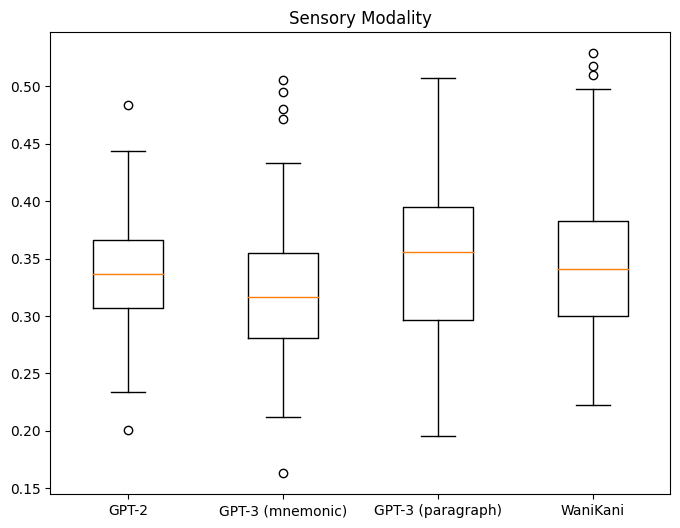
\includegraphics[width=400pt]{resources/ser_mean_box_plot.png}
    \caption{Sensory Modality Mean Scores}
    \label{figure:ser_mean_box_plot}
\end{figure}

\begin{figure}
    \centering
    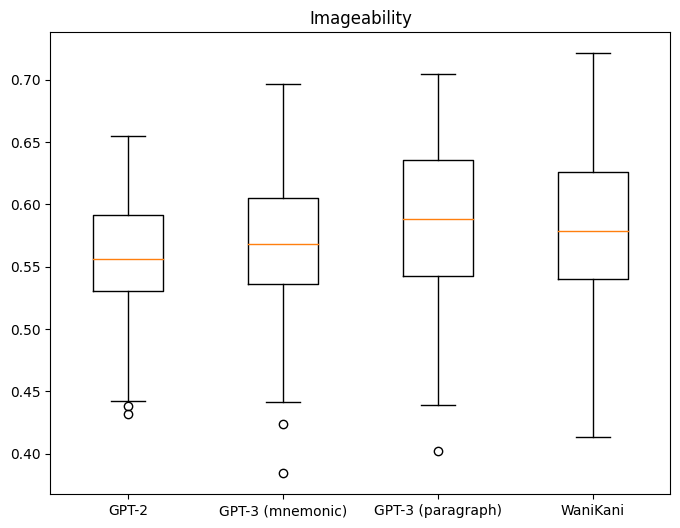
\includegraphics[width=400pt]{resources/img_mean_box_plot.png}
    \caption{Imageability Mean Scores}
    \label{figure:img_mean_box_plot}
\end{figure}

\begin{figure}
    \centering
    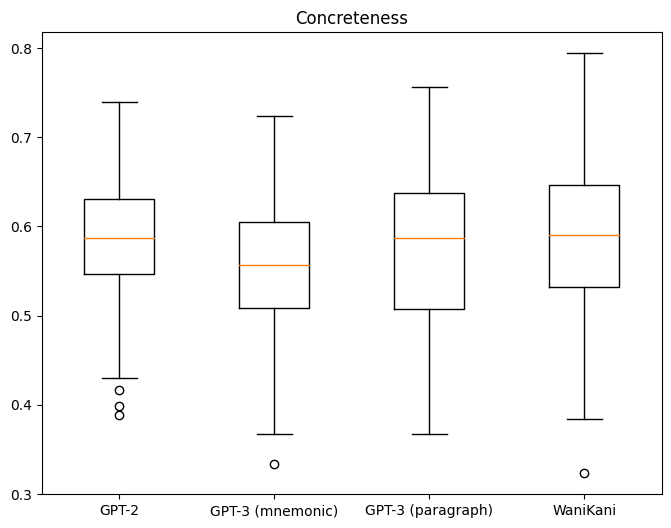
\includegraphics[width=400pt]{resources/concr_mean_box_plot.png}
    \caption{Concreteness Mean Scores}
    \label{figure:concr_mean_box_plot}
\end{figure}
The ANOVAS's for all features were significant ($p < 0.05$). However, the differences are not very striking and the significant interaction terms between groups often show the opposite trend of what I had hoped for. Namely the paragraphs from GPT-3 often and GPT-2 generated mnemonics often have a higher overall mean than GPT-3 mnemonics and the WaniKani mnemonics. I have also tried to use the $median$ and $maximum$ of mnemonic scores but the results are comparable and therefore of no further interest. Given these results I conclude that simple metrics like $mean$, $median$, and $maximum$ of language norm scores over all tokenized words of individual mnemonics aren't very useful in separating the groups.

As a next step I want to quantify the bizarreness of text to potentially separate the four groups. Based on the observation that bizarre language uses words that are not commonly found together we may get some estimate of how bizarre a mnemonic is, based on the probability of their content occurring. To clarify this the phrase "a horse and a tiger racing each other" is probably a lot less likely to occur than seeing the phrase "two cars racing each other". To get a value for how likely text is to occur I will use perplexity scalars. This metric was explained earlier in Chapter \ref{sec:body_state_of_the_art} (Equation \ref{eq:ppl}). One reason to be careful with this metric is that its measures are dependant on the training data and model architecture. For the experiment I used GPT-2 based perplexity which was trained with a dataset called WebText which was never fully published but contains mostly text from web pages that had been scraped by following outbound links from Reddit \cite{gpt2_hugging_face}. Results are shown in Table \ref{tab:ppl_whole_mnemonic} and plotted in Figure \ref{figure:ppl_whole_mnemonic}.     
\begin{table}[ht] 
\centering
\caption{Means and Standard Deviations for Perplexity}
\label{table:group_stats}
\begin{tabular}{lcc}
\toprule
Group & Mean & Standard Deviation \\
\midrule
GPT-2& $20.08$ & $12.71$ \\
GPT-3 (mnemonic) & $13.08$ & $4.30$ \\
GPT-3 (paragraph)& $22.63$ & $16.18$ \\
WaniKani & $36.13$ & $18.08$ \\
\bottomrule
\end{tabular}
\label{tab:ppl_whole_mnemonic}
\end{table}
\begin{figure}
    \centering
    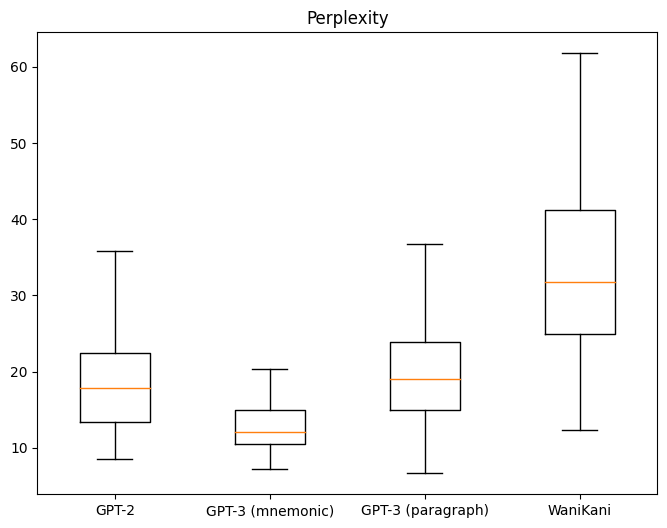
\includegraphics[width=400pt]{resources/ppl_entire_mnemonic.png}
    \caption{Perplexity Values}
    \label{figure:ppl_whole_mnemonic}
\end{figure}

As is evident, the ANOVA was highly significant ($p = 0.000$). We can also observe the promising clear shift between WaniKani mnemonics and all other groups. The difference between the GPT-2 XL mnemonics and the WaniKani ones, however, is alarming. Given that the former frequently contains incoherent phrases due to the beam search constrains, I would have expected their perplexity values to be much higher. Additionally the GPT-3 mnemonics have the overall lowest perplexity which renders the utility of perplexity for evaluating mnemonics questionable. The mnemonics by GPT-3 are storylike and often start with "Once upon a time". Perhaps the relatively low perplexity can be explained by taking a deeper look at the training data. It is possible that WebText contained a lot of story material. Moreover, the result may be explained by the model favoring output from other AI models over text written by humans. This poses an interesting question about the limitations of current language models that could be examined further. 

In order to reduce the overall bias towards different structures of text I chose to do second experiment. Instead of computing perplexity for the entire mnemonic, I tokenized the text into chunks of roughly $4$ words and then considered their mean. (Table \ref{tab:ppl_4_chunks}, Figure \ref{figure:ppl_4_chunks}) I should mention that for the Figures showing perplexity, outliers have been removed.
\begin{table}[ht] 
\centering
\caption{Means and Standard Deviations for Perplexity (Chunks)}
\label{table:group_stats}
\begin{tabular}{lcc}
\toprule
Group & Mean & Standard Deviation \\
\midrule
GPT-2& $2734$ & $6373$ \\
GPT-3 (mnemonic) & $703$ & $741$ \\
GPT-3 (paragraph)& $629$ & $361$ \\
WaniKani & $956$ & $592$ \\
\bottomrule
\end{tabular}
\label{tab:ppl_4_chunks}
\end{table}
\begin{figure}
    \centering
    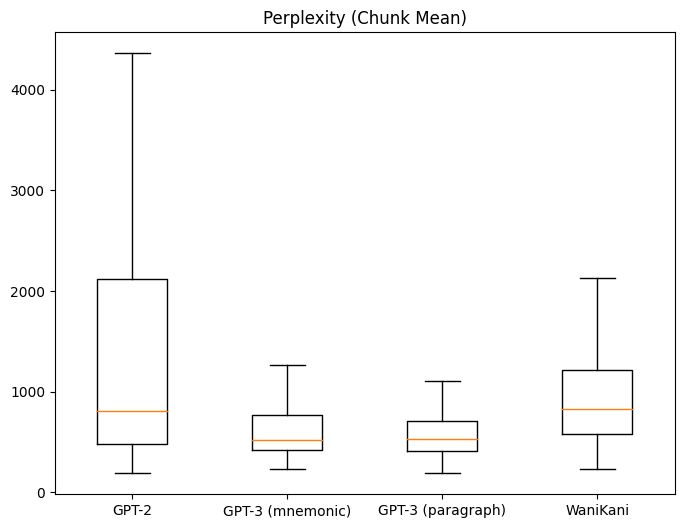
\includegraphics[width=400pt]{resources/ppl_4_chunks.png}
    \caption{Perplexity Values (Chunks)}
    \label{figure:ppl_4_chunks}
\end{figure}

The results turned out to be much more promising for the second attempt. As expected perplexity for GPT-2 mnemonics is now enormous and Wankani mnemonics are much more "perplexed" than the GPT-3 ones. Although not significant at all the mean of the GPT-3 mnemonics is now slightly higher than that of the paragrah ones. Overall, these numbers support the idea that perplexity is related to the bizarreness of language and should be considered to be included in the final metric. 

One baseline requirement for any generation method was to include all input words in the generated mnemonic. While all groups fulfill this baseline, a quick look at the data reveals that the significance of the input words in the corresponding mnemonic varies a lot. In short good mnemonics revolve around the input words. Given this insight it is plausible to utilize an exhaustive history of research on keyphrase extraction for the task of evaluating how central the input words are represented in the output. The idea is simple: input words should be keywords in mnemonics. Following I will benchmark 4 unsupervised keyword extraction algorithms for this task. I've come up with a recall based centrality score that leverages the scores for individual keyphrases.
\begin{equation}
    C(M, I) = \sum_{k \in E(M) \cap I} \frac{s(k)}{\sum_{k' \in E(M)} s(k')}
\end{equation}
The $E(M)$ represents the set of keyphrases extracted from the mnemonic. Only keyphrases that contain input words from $I$ are counted. They are weighted by the scores $s(k)$ given by the underlying extraction algorithm. These scores are then normalized.
YAKE and KPMiner are statistical models while TopicRank and MultipartiteRank are graph-based. Thanks to the \texttt{pke} \cite{pke} library the implementation of all algorithms is straightforward. The results are shown in Tables \ref{tab:yake_centrality}, \ref{tab:kpminer_centrality}, \ref{tab:topic_rank_centrality} and \ref{tab:multipartite_rank_centrality}.


\begin{table}[ht] 
\centering
\caption{Means and Standard Deviations for YAKE}
\label{table:group_stats}
\begin{tabular}{lcc}
\toprule
Group & M & SD\\
\midrule
GPT-2& $0.23$ & $0.22$ \\
GPT-3 (mnemonic) & $0.31$ & $0.18$ \\
GPT-3 (paragraph)& $0.32$ & $0.15$ \\
WaniKani & $0.40$ & $0.20$ \\
\bottomrule
\end{tabular}
\label{tab:yake_centrality}
\end{table}
\begin{table}[ht] 
\centering
\caption{Means and Standard Deviations for KPMiner}
\label{table:group_stats}
\begin{tabular}{lcc}
\toprule
Group & M & SD\\
\midrule
GPT-2& $0.31$ & $0.23$ \\
GPT-3 (mnemonic) & $0.42$ & $0.22$ \\
GPT-3 (paragraph)& $0.42$ & $0.21$ \\
WaniKani & $0.57$ & $0.22$ \\
\bottomrule
\end{tabular}
\label{tab:kpminer_centrality}
\end{table}
\begin{table}[ht] 
\centering
\caption{Means and Standard Deviations for TopicRank}
\label{table:group_stats}
\begin{tabular}{lcc}
\toprule
Group & M & SD\\
\midrule
GPT-2& $0.15$ & $0.11$ \\
GPT-3 (mnemonic) & $0.33$ & $0.13$ \\
GPT-3 (paragraph)& $0.30$ & $0.13$ \\
WaniKani & $0.42$ & $0.14$ \\
\bottomrule
\end{tabular}
\label{tab:topic_rank_centrality}
\end{table}
\begin{table}[ht] 
\centering
\caption{Means and Standard Deviations for MultipartiteRank}
\label{table:group_stats}
\begin{tabular}{lcc}
\toprule
Group & M & SD\\
\midrule
GPT-2& $0.15$ & $0.11$ \\
GPT-3 (mnemonic) & $0.35$ & $0.14$ \\
GPT-3 (paragraph)& $0.31$ & $0.14$ \\
WaniKani & $0.47$ & $0.15$ \\
\bottomrule
\end{tabular}
\label{tab:multipartite_rank_centrality}
\end{table}
All ANOVAS's have been highly significant. As can be seen, all algorithms show a similar trend that is very promising. Overall the graph-based algorithms are slightly better and MultipartiteRank was the only one that had a significant interaction between GPT-3 mnemonics and paragraphs, favoring the former as expected. The best results are plotted in Figure \ref{figure:mpr_centrality}. I suspect that the statistical models are better suited for larger text samples as word frequency is an important feature for identifying keyphrases. The graph-based models are perhaps better at capturing these strong connection as I described them earlier since graphs allow the models to represent semantic relationships between words and phrases. Another simpler explanation could be that the difference between the two paradigms is due to the fact I can set POS tags considered as keywords for the graph-based algorithms. By default VERBs are not included, which is why I added them. This option was not available however for the statistical models at least in the implementations provided by \texttt{pke}. 
\begin{figure}
    \centering
    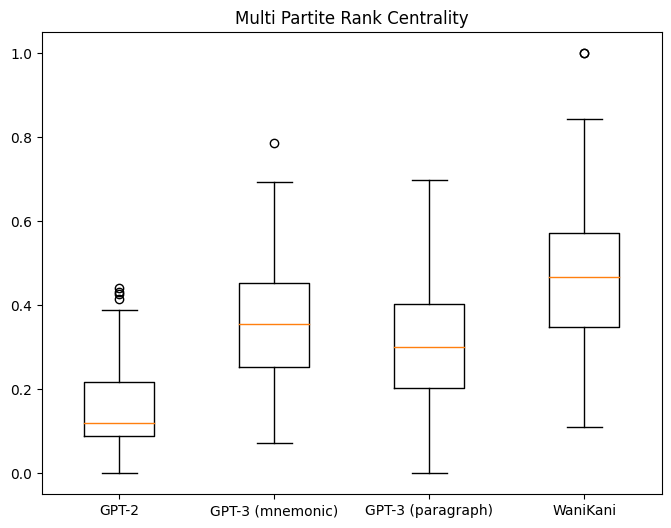
\includegraphics[width=400pt]{resources/mpr_centrality.png}
    \caption{MultipartiteRank Centrality Means}
    \label{figure:mpr_centrality}
\end{figure}

Given the success of matching the overlap of keywords and input words led me to question whether the linguistic features sensory modality, imageability and concreteness could significantly separate the groups if they were applied only to the keywords. All of these tests had been statistically insignificant as well. However limiting the number of evaluated keywords to the length of the input words had a significant effect for concreteness and imageability. Despite this I decided to exclude their contribution to the final metric as the only way to get a perfect score would require the input word imageability ratings to all equal 1. So instead of getting an estimate of how imageable the mnemonic is, you would instead get a scalar that indicates how imageable the top $n$ keywords are, which ideally are the input words and therefore I'd simply rate the imageability of the input words. Since the quality of the mnemonic should be independant of the input words I attempted to only score the imageability of the top $n$ keywords ($n = len(\text{input words})$) that do not include any input words. While these keywords may not include the input words, they could perhaps still be complementary to them and therefore be more vivid. This turned out to be insignificant as well.

To conclude this chapter I propose a simplified metric that is essentially equivalent to \emph{recall}. Based on my previous findings (Figure \ref{figure:mpr_centrality} Multipartite Rank is used to extract keywords from the mnemonics and the score is simply the proportion of keywords that includes input words. Once an input word is found in the mnemonic it is only counted once. 
\begin{equation}
    S(K, I) = \frac{\sum_{i=1}^{|I|} 1(k_i \in I)}{|I|}
\end{equation}
This metric is closer to the initial hypothesis, namely, the set of $n$ top keywords should be the set of input words. It is also simpler as it does not depend on the weights of the underlying keyword extraction algorithm. Most importantly, it does a great job at separating the groups. The results are found in Table \ref{tab:final_metric_recall} and Figure \ref{figure:recall}.
\begin{table}[ht] 
\centering
\caption{Means and Standard Deviations for Recall}
\label{table:group_stats}
\begin{tabular}{lcc}
\toprule
Group & M & SD\\
\midrule
GPT-2& $0.18$ & $0.22$ \\
GPT-3 (mnemonic) & $0.51$ & $0.25$ \\
GPT-3 (paragraph)& $0.37$ & $0.24$ \\
WaniKani & $0.66$ & $0.26$ \\
\bottomrule
\end{tabular}
\label{tab:final_metric_recall}
\end{table}
\begin{figure}
    \centering
    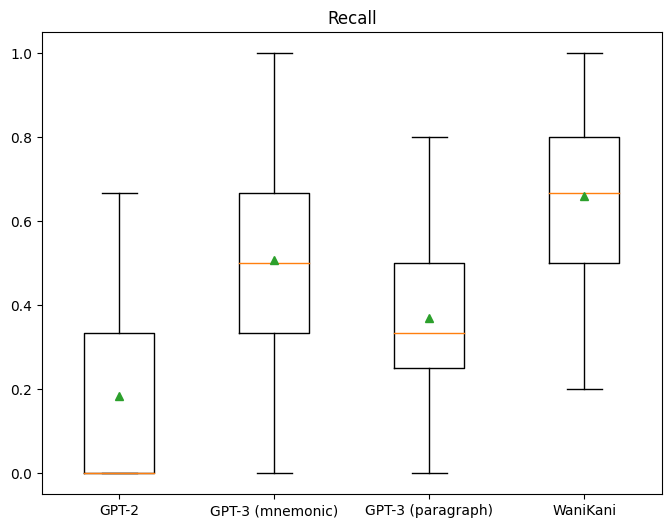
\includegraphics[width=400pt]{resources/recall.png}
    \caption{Recall}
    \label{figure:recall}
\end{figure}







\subsection{Footnotes and References} \label{sec:body_refs}

References to external work are your way provide additional information to the reader.

Footnotes are used for any information that isn't crucial for the text but could be used by a more interested reader to get more information \footnote{It's a good idea to keep them short and to the point}. They may also contain links \footnote{e.g., to \url{http://isitfriday.org}}.

References are your way to refer to existing scientific work. They shouldn't be limited to the state of the art section. They can be used whenever you want to establish a fact that has already been published or if you want to point the reader to a place where they can find additional information.
Throughout your thesis you should include keys to the respective publications right after you use content from them. For example, this would look like this: \cite{greenwade93} \cite{einstein} .


\subsection{Tables and Figures} \label{sec:body_tables}

